% This is samplepaper.tex, a sample chapter demonstrating the
% LLNCS macro package for Springer Computer Science proceedings;
% Version 2.21 of 2022/01/12
%
\documentclass[runningheads]{llncs}
%
\usepackage[T1]{fontenc}
% T1 fonts will be used to generate the final print and online PDFs,
% so please use T1 fonts in your manuscript whenever possible.
% Other font encondings may result in incorrect characters.
%
\usepackage{graphicx}
\usepackage{amssymb}
\usepackage{color}
\usepackage{graphics}
% Used for displaying a sample figure. If possible, figure files should
% be included in EPS format.
%
% If you use the hyperref package, please uncomment the following two lines
% to display URLs in blue roman font according to Springer's eBook style:
%\usepackage{color}
%\renewcommand\UrlFont{\color{blue}\rmfamily}
%\urlstyle{rm}
%
\begin{document}
	
	\title{Learning Heuristics for Multiple Gapped Longest Common Subsequence Problem}
	%
	\titlerunning{ MGLCSP}
	
	\author{Marko Djukanović\inst{1} 
	}
	%
	\authorrunning{Djukanovic et al.}
	
	\institute{ University of Nova Gorica, Nova Gorica, Slovenia \\ \email{marko.dukanovic@ung.si}  
	}
	%
	\maketitle              %  
 
	\vspace{-0.5cm}
    \begin{abstract}
    	Combinatorial optimization problems over sequences are central in bioinformatics, text processing, and other computational domains. One of  them, the \textit{Variable Gapped Longest Common Subsequence Problem} (VGLCSP)~\cite{penga2011longest} poses significant computational challenges due to the exponential growth of the search space with the number of sequences and variable gap constraints. Traditional exact algorithms, while guaranteeing optimal solutions, are impractical for medium-to-large instances, whereas heuristic approaches often rely on static scoring functions that fail to exploit structural patterns across diverse problem instances.
    	
    	In this work, we propose a data-driven framework to construct a learning-based heuristic for guiding Beam Search (BS) in the VGLCSP~\cite{djukanovic_eurocast_2026}. The core idea is to combine a \textit{feed-forward neural network} (FFNN) with an \textit{Iterative Multi-Source BS} (IMSBS) algorithm, where the network learns to evaluate candidate extensions and guide the search toward high-quality subsequences. Unlike gradient-based approaches, the network weights are optimized using a \textit{Genetic Algorithm} (GA), such as standard Random Key GA (RKGA) and/or a biased RKGA (BRKGA) variant~\cite{gonccalves2011biased}. Each individual in the GA population represents a full set of network parameters, and its fitness is measured by embedding the NN within IMSBS and evaluating the average solution quality on a set of training instances. Validation instances are used exclusively for generalization monitoring.
    	
    	A key contribution of this work is the design of \textit{compact, instance-independent feature representations} for partial solutions. Each node in the search tree is encoded by a vector that captures: (i) normalized positions of the current matches in each sequence, summarized by maximum, minimum, mean, and standard deviation; (ii) the current length of the partially constructed subsequence; and (iii) statistics of remaining gap constraints, including minimum, maximum, mean, and standard deviation for each sequence of considered subproblem. Additional global instance features, such as the alphabet size $|\Sigma|$ and the number of sequences $m$, can also be appended. Altogether, these features create a low-dimensional yet expressive representation of the search state, enabling the NN to generalize across instances of varying size and complexity. %Different feature configurations allow exploration of trade-offs between compactness and expressiveness.
    	
    	The GA-based optimization process leverages evolutionary principles, including elitism, mutation via random immigrants, and multiple offspring generation strategies (RKGA or BRKGA). The best-performing individual at each generation guides the BS heuristic, and the overall framework alternates between network optimization and search evaluation, forming a tightly coupled neuro-evolutionary hyper-heuristic. This approach allows learning in fully \textit{non-differentiable} settings, as the network is never trained to directly predict solutions but rather to \textit{guide} the search toward promising candidates.  
        \vspace{-0.7cm}
    	\begin{figure}[!ht]
    		\centering
    		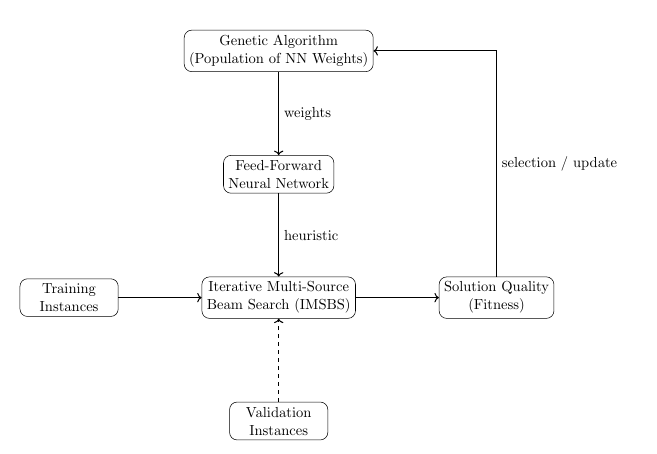
\includegraphics[width=150pt,height=100pt]{ffnn_train.png}
    		\caption{Graphical representation of learning NN-guidance} \vspace{-0.3cm}
    		\label{fig:ga_imsbs}
    	\end{figure}
    	To visualize the learning pipeline, Figure~\ref{fig:ga_imsbs} illustrates these interactions. % between GA, FFNN, IMSBS, training instances, and fitness evaluation. 
       The neural network outputs heuristic scores for IMSBS, which constructs partial subsequences.  Solution quality is then fed back into the GA to evolve the network weights, creating an adaptive loop that continuously improves search performance. Validation instances are processed only for monitoring purposes, ensuring that the learned heuristics generalize beyond the training set.
    	
    	Preliminary experiments demonstrate that the learning-based IMSBS (LIMSBS) can match or outperform state-of-the-art IMSBS across a variety of instance categories, characterized by sequence number $m \in \{2,3,5,10\}$, sequence length $n \in \{50,100,200,500\}$, and alphabet size $|\Sigma| \in \{2,4\}$. {The neural network configuration providing the best performance employs a three-layer architecture with 10 neurons and  \texttt{ReLU} activation on each layer,  incorporating both instance-level features and alphabet size.} Even under a modest training budget of two hours for BRKGA, LIMSBS exhibits improved average objective values over IMSBS for larger $m\leq 5$, highlighting the potential of data-driven heuristics for scaling BS to complex VGLCS instances.
    	
    	In summary, this work presents a generalizable, learning-augmented Beam Search framework for the VGLCSP, integrating evolutionary optimization with neural network heuristics. The proposed method advances the state-of-the-art by enabling adaptive guidance of combinatorial search in non-differentiable and high-dimensional settings, demonstrating both improved solution quality and robustness across diverse instances. Our approach offers a blueprint for applying neuro-evolutionary hyper-heuristics to a broader class of combinatorial optimization problems where explicit heuristic design is difficult or infeasible.
    \end{abstract}
    Acknowledgments. TODO
	
	\bibliographystyle{splncs04}
	\bibliography{bib}
	%
	
\end{document}